\documentclass[a4paper, 11pt, oneside]{book}
\usepackage{/home/nicolas/Documents/Enseignement/Prepa/bpep/fichiers_utiles/preambule}

\newcommand{\dsNB}{2}
\makeatletter
\renewcommand{\@chapapp}{Kh\^olles MPSI3 -- semaine \dsNB}
\makeatother

\toggletrue{corrige}  % décommenter pour passer en mode corrigé

\begin{document}

\resetQ
\newpage

\chapter{Sujet 1\siCorrige{\!\!-- corrigé}}
\section{Question de cours}

Construire l'image d'un objet après le centre optique d'une lentille
convergente, précisez la nature de l'objet et de l'image. Construire le rayon
émergent d'un rayon quelconque pour une lentille divergente en présentant les
règles de construction secondaires et nommant tous les points d’intérêt.

\section{Étude d'un rétroprojecteur}
\begin{wrapfigure}[10]{R}{.4\linewidth}
    \vspace*{-18pt}
    \centering
    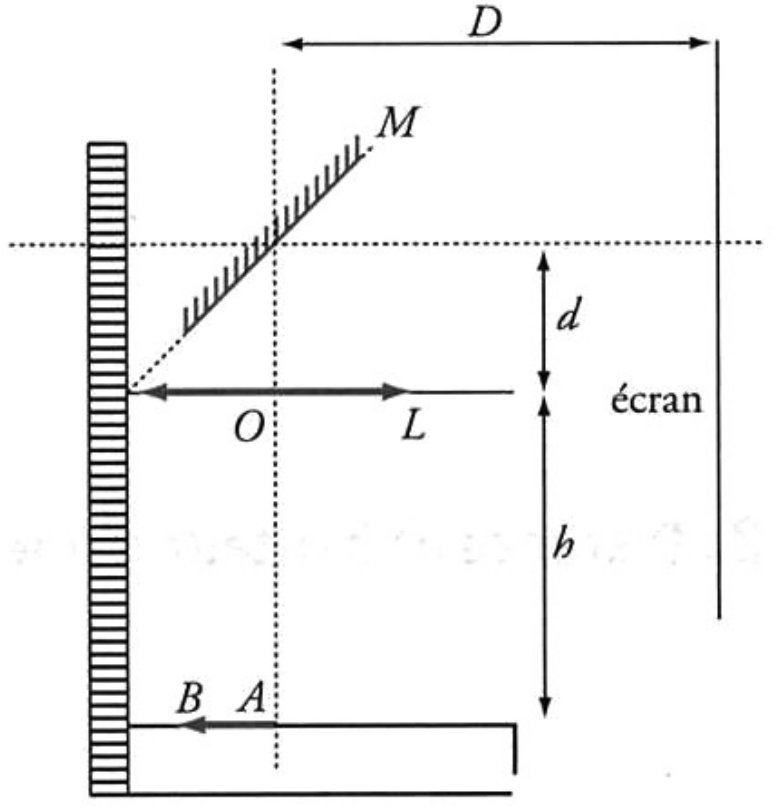
\includegraphics[width=.5\linewidth]{retro}
    \caption{Schéma du rétroprojecteur}
    \label{fig:retro}
\end{wrapfigure}

Un rétroprojecteur est un ensemble lentille-miroir, avec un miroir plan incliné
à \ang{45;;} par rapport à la lentille. L'ensemble lentille-miroir est réglable
en hauteur ($h$). On étudie un rétroprojecteur dont la lentille a une vergence
de $\SI{2.0}{\delta}$, avec une distance lentille-miroir $d = \SI{10}{cm}$. 

On désire projeter un objet transparent $AB$ sur un écran placé à $D =
\SI{3.0}{m}$ de l'axe optique de la lentille.

\QR{Déterminer la distance $h$ permettant d'obtenir une image nette sur
l'écran.}{On a $AB \opto{\Lc}{O} A_1B_1 \opto{M}{H} A'B'$, avec $H$ le point
        d'intersection entre le miroir plan et l'axe optique de la lentille.
        L'image finale $A'$ donnée par le miroir plan est telle que
        \begin{empheq}[box=\fbox]{equation*}
            \obar{HA'} = \obar{HA_1} = D
        \end{empheq}
        On a donc pour la lentille
        \begin{empheq}[box=\fbox]{align*}
            \obar{OA_1} &= \obar{OH} + \obar{HA_1}\\
            \Leftrightarrow \obar{OA_1} &= d+D
        \end{empheq}
        On utilise la relation de conjugaison des lentilles minces en nommant
        $V$ la vergence de la lentille~:
        \begin{equation*}
            V = \frac{1}{d+D} - \frac{1}{-h} \Leftrightarrow
            \boxed{h = \frac{d+D}{V(d+D)-d}}
            \quad\text{avec}\quad
            \left\{
                \begin{array}{rcl}
                    d & = & \SI{10e-2}{m}\\
                    D & = & \SI{3.0}{m}\\
                    V & = & \SI{2.0}{m^{-1}}
                \end{array}
            \right.
        \end{equation*}
        Et l'application numérique donne
        \begin{equation*}
            \boxed{h = \SI{60}{cm}}
    \end{equation*}}
    \QR{Calculer le grandissement.}{
    Le miroir plan a un grandissement de 1, donc le grandissement du
        système est celui de la lentille~: on a $\gamma = \DS
        \frac{\obar{A_1B_1}}{\obar{AB}} = \frac{\obar{OA_1}}{\obar{OA}}$, soit
        \begin{empheq}[box=\fbox]{align*}
            \gamma &= \frac{d+D}{-h}\\
            \gamma &= -5.2
        \end{empheq}
}

\resetQ

\newpage

\chapter{Sujet 2\siCorrige{\!\!-- corrigé}}
\section{Exercice de cours~: condition de netteté}

\QR{Soit $AB \opto{\Lc}{O} A'B'$ avec $\Lc$ convergente projetant sur un écran. On
appelle $x$ la distance $ \left| \OA \right|$ et $D$ la distance fixe $AA'$.
Quelle est la contrainte sur le choix de lentille pour que $A'B'$ soit nette~?}{
\begin{tcbraster}[raster columns=2, raster equal height=rows]
    \begin{NCdefi}[]{Données}
        \begin{center}
            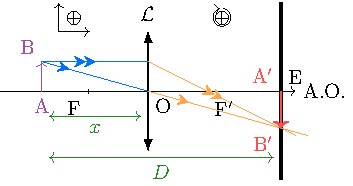
\includegraphics[width=\linewidth]{../figures/lent_conv-condition.pdf}
            \captionof{figure}{Schéma de situation}
            \label{fig:lent_condi}
        \end{center}
    \end{NCdefi}
    \begin{tcolorbox}[blankest, raster multicolumn=1]
        \begin{tcbraster}[raster columns=1]
            \begin{NCprop}[]{Résultat attendu}
                L'image est nette si la lentille forme l'image sur l'écran. Avec
                $D$ fixe, on cherche une équation avec $x$.
            \end{NCprop}
            \begin{NCrapp}[]{Outils}
                Relation de Descartes
                \[\boxed{ \frac{1}{\OF} = \frac{1}{\OAp} - \frac{1}{\OA}}\]
                et $\OA = -x$, $\OAp = D-x$.
            \end{NCrapp}
        \end{tcbraster}
    \end{tcolorbox}
\end{tcbraster}

\begin{NCexem}[sidebyside]{Application}
    Avec les notations de l'énoncé, la relation de Descartes devient
    \begin{align*}
        \frac{1}{f'} &= \frac{1}{D-x} - \frac{1}{-x}\\
        \Leftrightarrow \frac{1}{f'} &= \frac{x + D-x}{x(D-x)}\\
        \Leftrightarrow f' &= \frac{x(D-x)}{D}\\
        \Leftrightarrow 0 &= x^2 - xD + f'D 
    \end{align*}
    \tcblower
    Ce trinôme du second degré a pour discriminant $\Delta = D^2-4f'D =
    D(D-4f')$. $x$ étant une distance physique, on cherche $\Delta \geq 0$.
    \begin{itemize}
        \item $\Delta = 0$ si $D = 4f'$, et alors \[\boxed{x = \frac{D}{2}}\]
        \item $\Delta > 0$ si $D > 4f'$, et alors \[\boxed{x_\pm =
            \frac{D\pm\sqrt{D(D-4f')}}{2}}\]
    \end{itemize}
    Ainsi, la zone de netteté de l'image se situe entre $x_+$ et $x_-$, et a
    donc une largeur $d = x_+ - x_- = \sqrt{D(D-4f')}$.
\end{NCexem}}

\resetQ
\section{Grenouille intelligente}

Pour se cacher des prédateurs, une grenouille s'est accrochée sous un nénuphar
qui flotte sur l'étang. La grenouille a une hauteur $h$ et le nénuphar un rayon
$R$ et une épaisseur très faible.

\QR{Quel doit être le rayon minimal $R_0$ du nénuphar pour que les pieds de la
grenouille ne soient pas visibles par un prédateur situé en-dehors de l'eau?}{
\begin{tcbraster}[raster columns=7, raster equal height=rows]
    \begin{NCdefi}[raster multicolumn=4]{Données}
        Pour une hauteur de grenouille fixée, il y a une taille de
        nénuphar permettant à tous les rayons partant de la grenouille de ne
        pas traverser le dioptre.\smallbreak
        \begin{center}
            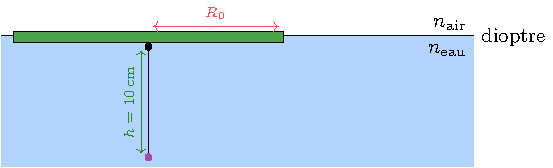
\includegraphics{../figures/ch2-2-1}   
        \end{center}
    \end{NCdefi}
    \begin{tcolorbox}[blankest, raster multicolumn=3, space to=\myspace]
        \begin{tcbraster}[raster columns=1]
            \begin{NCprop}{But à atteindre}
                Origine physique de ce phénomène et traduction mathématique.
            \end{NCprop}    
            \begin{NCrapp}{Outils du cours}
                Loi de Snell-Descartes :
                \[ n_1\sin i_1 = n_2\sin i_2\]
                et \underline{angle limite} de réfraction, tel que
                \[ n_1\sin i_\ell = n_2\sin \ang{90;;} = n_2\]
                qui indique que pour $n_1 > n_2$, il y a un angle d'incidence à
                partir duquel il n'y a pas de rayon réfracté (les rayons
                réfractés font un angle de 90° avec la normale et sont donc
                parallèles au dioptre).
            \end{NCrapp}
        \end{tcbraster}
    \end{tcolorbox}
\end{tcbraster}
\begin{NCexem}[breakable]{Application}
    Pour que les pieds de la grenouille ne soient pas visibles par un prédateur
    situé en-dehors de l'eau, c'est-à-dire au-dessus du dioptre, il faut
    simplement qu'il n'y ait pas de rayon partant de ses pieds et qui puissent
    sortir de l'eau : il faut que tous les rayons avec un angle d'incidence plus
    faible que cet angle limite soient bloqués par le nénuphar. C'est possible
    puisqu'on est dans une situation où le rayon passe dans un milieu
    \textbf{moins réfringent}, i.e. $n_2 < n_1$. En effet, dans cette situation
    il y a une inclinaison du rayon incident qui implique que le rayon émergent
    est parallèle à la surface, et tous les rayons au-delà de cet angle limite
    sont tous réfléchis. Un beau, grand schéma avec toutes les données reportées
    dessus mène naturellement à l'utilisation de formules trigonométriques de
    4\ieme.
    \begin{center}
        \vspace*{-2.5cm}
        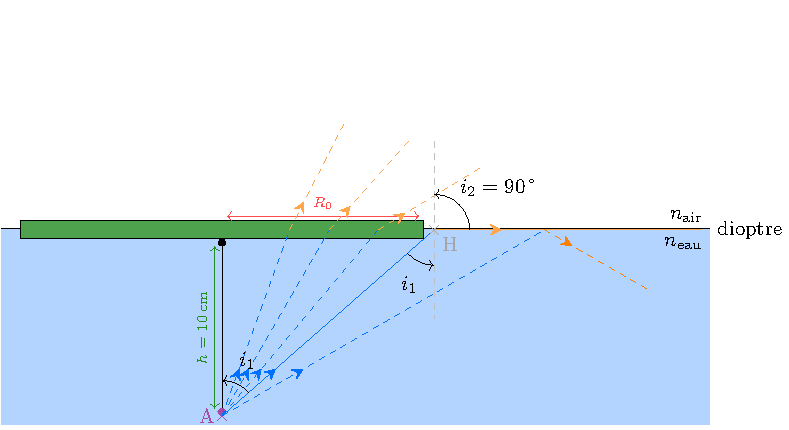
\includegraphics{../figures/ch2-2-2}
    \end{center}
    On voit ici qu'une simple fonction $\tan$ permet d'exprimer $R_0$ :
    \begin{empheq}[box=\fbox]{align}\label{eq:tan}
        \tan i_1 = \frac{R_0}{h}
    \end{empheq}
    Seulement on n'a pas encore la valeur de $i_1$. Or, on a déterminé que pour
    fonctionner l'astuce de la grenouille est d'avoir $i_1 = i_\ell$, et d'après
    le cours :
    \begin{empheq}{align}
        n\eau\sin i_\ell       & = n\air\\
        \Leftrightarrow i_\ell & = \asin \frac{n\air}{n\eau}\label{eq:ilim}
    \end{empheq}
    On peut donc écrire, avec \ref{eq:tan} et \ref{eq:ilim} :
    \begin{empheq}[box=\fbox]{equation}
        R_0 = h\times\tan\left(\asin \frac{n\air}{n\eau}\right)
        \quad \text{avec}
        \left\{
            \begin{array}{rcl}
                h & = & \SI{10.0}{cm}\\
                n_\mathrm{air} & = & \num{1.00}\\
                n_\mathrm{eau} & = & \num{1.33}
            \end{array}
        \right.
    \end{empheq}
    et finalement,
    \begin{empheq}[box=\fbox]{equation}
        R_0 = \SI{11.4}{cm}
    \end{empheq}
\end{NCexem}
}

%\subimport{/home/nicolas/Documents/Enseignement/Prepa/bpep/exercices/Colle/Capteur_de_niveau_d_eau/}{sujet.tex}

\resetQ
\newpage

\chapter{Sujet 3\siCorrige{\!\!-- corrigé}}
\section{Question de cours}

\QR{On modélise l'objectif d'un vidéoprojecteur par une lentille mince convergente
de distance focale de \SI{5.0}{cm}. L'objet transverse a une hauteur de
\SI{24}{mm} et l'écran se situe à \SI{4.0}{m} de la lentille. Déterminer la
position, la nature de l'objet ainsi que la taille de l'image.}{
\begin{NCdefi}[sidebyside, sidebyside align=center]{Données}
    \begin{enumerate}
        \item $(AB) = \SI{24}{mm}$ : « l'objet est une matrice de $ \SI{24}{mm}$
            » ;
        \item $ \obar{OA'} = \SI{+4.0}{m}$ : « l'écran se situe à $\SI{4.0}{m}$ »
            (c'est là que se forme l'image, c'est donc la position de $A'$) ;
        \item $ \obar{OF'} = \SI{+5.0}{cm}$.
    \end{enumerate}
    \tcblower
    \begin{center}
        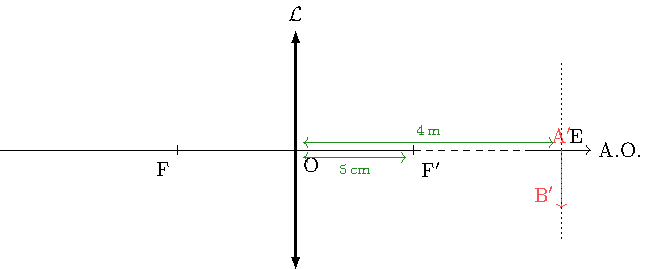
\includegraphics[width=\linewidth]{videoproj_plain.pdf}
    \end{center}
\end{NCdefi}
\begin{tcbraster}[raster columns=2, raster equal height=rows]
    \begin{NCprop}{Résultats attendus}
        \begin{enumerate}
            \item Que vaut $ \obar{OA}$ ? : « Déterminer la position et la nature de
                l'objet » ($O$ est bon point d'intérêt à partir duquel on peut
                mesurer des distances, et selon la valeur \underline{algébrique} de
                $\obar{OA}$ on saura de quel côté de la lentille l'objet se situe,
                et donc son caractère virtuel ou réel) ;
            \item Que vaut $\ABp$ ? : « Déterminer [...] la taille de l'image ».
        \end{enumerate}
    \end{NCprop}
    \begin{NCrapp}{Outils du cours}
        \begin{enumerate}
            \item Relation de conjugaison pour une lentille mince :
                \[ \boxed{ \frac{1}{\OF} = \frac{1}{\OAp} - \frac{1}{\OA}}\]
            \item Grandissement pour une lentille mince
                \[\boxed{\g = \frac{\ABp}{\ABb} = \frac{\OAp}{\OA}}\]
        \end{enumerate}
    \end{NCrapp}
\end{tcbraster}
\begin{NCexem}[breakable, sidebyside]{Application}
    \begin{enumerate}
        \item De la relation de conjugaison, on a :
            \[\OA = \left[ \frac{1}{\OAp} - \frac{1}{\OF} \right]^{-1}\]
            Et avec les données,
            \[ \boxed{\OA = \SI{- 5.0}{cm}}\]
            Ainsi, on a un \underline{objet réel} situé à 5 centimètres à gauche de
            la lentille.

        \item De l'expression du grandissement, on a
            \[\ABp = \ABb\times\frac{\OAp}{\OA}\]
            Et avec les données,
            \[ \boxed{\ABp = \SI{- 1.9}{m}} \]
    \end{enumerate}
    \tcblower
    \begin{center}
        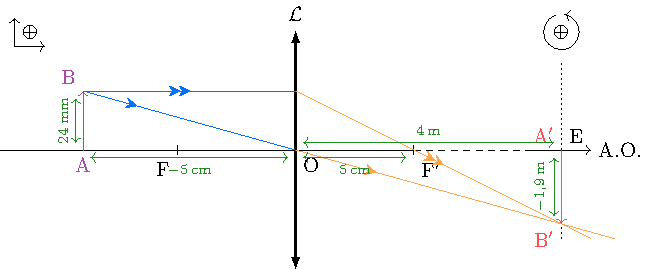
\includegraphics[width=\linewidth]{videoproj.pdf}
    \end{center}
\end{NCexem}}

\resetQ

\section{Prisme rectangle}

\QR{On utilise un prisme de verre d'indice $n=\num{1.5}$. Sa section principale
    est un triangle $ABC$ rectangle en $A$ tel que l'angle en $B$ soit égal à
    \ang{70;;}. Un rayon lumineux dans le plan $ABC$ rencontre le prisme en $I$
    sur le côté $AB$ perpendiculairement à $AB$. Sachant que le rayon incident
    est dans l'air, étudier la marche de la lumière jusqu'à la sortie du
prisme.}{
\begin{tcbraster}[raster columns=3, raster equal height=rows]
    \begin{NCdefi}[raster multicolumn=2]{Schéma}
        \begin{center}
            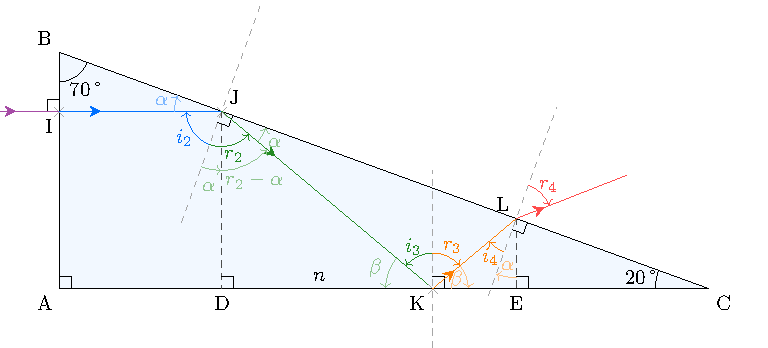
\includegraphics[scale=0.94]{../figures/ch2-9}
            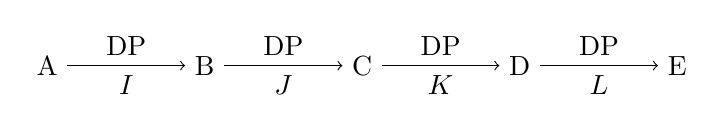
\begin{tikzpicture}[]
                \node[] (A) at (0,0) {A};
                \node[] (B) at (2,0) {B};
                \node[] (C) at (4,0) {C};
                \node[] (D) at (6,0) {D};
                \node[] (E) at (8,0) {E};
                \draw[->] (A) -- (B)
                    node [midway, above] {DP}
                    node [midway, below] {$I$};
                \draw[->] (B) -- (C)
                    node [midway, above] {DP}
                    node [midway, below] {$J$};
                \draw[->] (C) -- (D)
                    node [midway, above] {DP}
                    node [midway, below] {$K$};
                \draw[->] (D) -- (E)
                    node [midway, above] {DP}
                    node [midway, below] {$L$};
            \end{tikzpicture}
        \end{center}
    \end{NCdefi}
    \begin{tcolorbox}[blankest, raster multicolumn=1, space to=\myspace]
        \begin{tcbraster}[raster columns=1]
            \begin{NCprop}[]{Résultat attendu}
                On cherche à suivre le chemin du rayon indiqué dans l'énoncé. Il
                faut pour cela savoir ce qui peut arriver au rayon. Dans le cas
                du passage par un dioptre plan, il peut y avoir traversée du
                dioptre avec Snell-Descartes, ou réflexion dans le cas $n_2 <
                n_1$.
            \end{NCprop}
            \begin{NCrapp}{Outils du cours}
                Loi de Snell-Descartes :
                \[ n_1\sin i = n_2\sin r\]
                et pour $n_2 < n_1$, $i_\ell$ :
                \[ n_1\sin i_\ell = n_2\sin \ang{90;;} = n_2\]
                tel que $i_1 > i_\ell$ est réfléchi.
            \end{NCrapp}
        \end{tcbraster}
    \end{tcolorbox}
\end{tcbraster}
\begin{NCexem}[sidebyside]{Application}
    Ici, l'angle limite de réflexion à l'intérieur du prisme est : \[i_\ell =
    \arcsin \frac{1}{n} = \boxed{ \ang{41.8;;}}\]
    \begin{description}
        \item[I] : $\boxed{i_1 = \ang{0;;}}$ donc
            $\boxed{r_1 = \ang{0;;}}$ ;
        \item[J] : Ici, on doit voir que $\alpha = \ang{20;;}$ puisque
            dans le triangle BIJ, la somme des angles doit valoir $\ang{180;;}$
            et qu'on a un angle droit + un angle de \ang{70;;}.
            On en déduit que $\boxed{i_2 = \ang{70;;}}$ également, car
            $i_2 + \alpha = \ang{90;;}$.\smallbreak
            Comme \underline{$i_2 > i_\ell$}, le rayon ne traverse pas mais est
            réfléchi, soit $\boxed{r_2 = \ang{70;;}}$.
    \end{description}
    \tcblower
    \begin{description}
        \item[K] : Pour trouver l'angle en K, on peut par exemple chercher
            l'angle $\beta$ : en construisant le triangle rectangle JDK, on
            trouve que l'angle au sommet est $r_2 - \alpha = \ang{50;;}$ ;
            avec l'angle droit en D, $\beta = \ang{40;;}$, et $\boxed{i_3
            = \ang{50;;} > i_\ell}$ donc rayon réfléchi $\boxed{r_3 =
        \ang{50;;}}$.
        \item[L] : De même qu'en J, tracer LEC indique que $i_4 + \alpha + \beta
            = \ang{90;;}$, soit $\boxed{i_4 = \ang{30;;} < i_\ell}$
            : on applique donc Snell-Descartes ici, et on obtient
            \[\boxed{r_4} = \arcsin (n\times \sin i_4) =
            \boxed{\ang{48.6;;}}\]
    \end{description}
\end{NCexem}

}

\resetQ

\chapter{Sujet 4\siCorrige{\!\!-- corrigé}}
\section{Exercice de cours~: champ de vision à travers un miroir plan}

Une personne dont les yeux se situent à $h = \SI{1.70}{m}$ du sol observe une
mare gelée (équivalente à un miroir plan) de largeur $l = \SI{5.00}{m}$ et
située à $d = \SI{2.00}{m}$ d'elle.

\QR{Peut-elle voir sa propre image~? Quelle est la nature de l'image~?}{
\begin{NCdefi}{Schéma}
    \begin{center}
        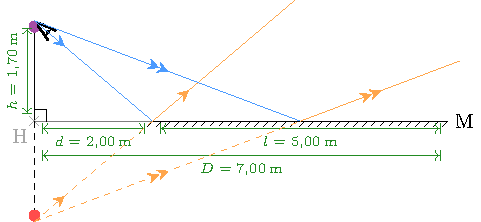
\includegraphics[width=\linewidth]{../figures/ch3-arbre-1}
    \end{center}
\end{NCdefi}
\begin{tcbraster}[raster columns=2, raster equal height=rows]
    \begin{NCrapp}{Outil}
        Pour voir une image, il faut qu'un rayon partant de l'image
        puisse arriver jusqu'à l'œil de l'observataire. Étant donné
        qu'on travaille avec un miroir, l'image de l'observataire est
        son symétrique par le plan du miroir (même si le miroir ne
        s'étend pas jusque-là !).
    \end{NCrapp}
    \begin{NCexem}{Application}
        On voit vite qu'il n'est pas possible qu'un rayon issu de
        l'image (en rouge) atteigne l'œil (en violet). On comprend par
        le tracé des rayons réfléchis que seul l'autre côté du lac sera
        visible.
    \end{NCexem}
\end{tcbraster}}
\QR{Quelle est la hauteur maximale $H$ d'un arbre situé de l'autre côté de la
    mare (en bordure de mare) qu'elle peut voir par réflexion dans la mare~? On
notera $D = l+d$.}{
\begin{NCdefi}{Schéma}
    \begin{center}
        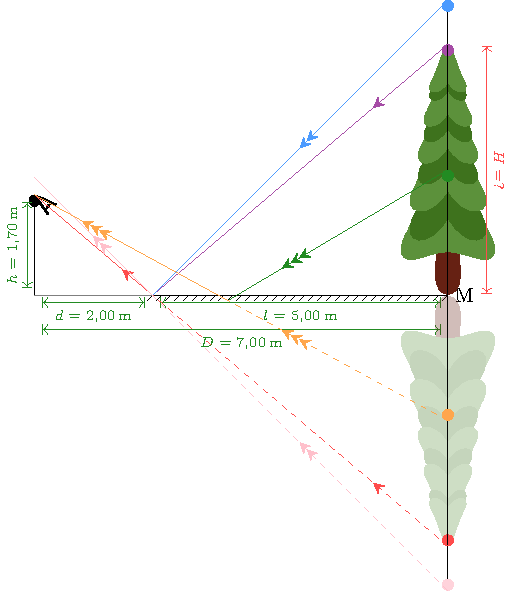
\includegraphics[width=.7\linewidth]{../figures/ch3-arbre-2}
    \end{center}
\end{NCdefi}
\begin{NCrapp}[]{Outil}
    Ici aussi, l'idée est de trouver l'image de l'arbre, et de voir
    la condition limite pour la taille visible.
\end{NCrapp}
\begin{NCexem}{Application}
    Un schéma avec l'image de l'arbre nous permet de voir que le
    point le plus haut qu'on peut voir par réflexion sur le lac est
    quand on regarde proche de nous : si on regarde plus loin, on
    voit en effet plus vers le bas de l'arbre (rayon vert incident,
    rayon orange émergent). Un arbre qui est trop grand ne sera pas
    visible en regardant ce point-là (rayon bleu incident, rose
    émergent). On s'intéresse donc à la construction géométrique
    formée par le rayon violet incident, rouge émergent, qui nous
    permet d'appliquer le théorème de Thalès : $\DS\frac{H}{l} =
    \frac{h}{d}$, soit
    \[\boxed{H = \frac{l\times h}{d}} \quad \text{avec} \quad
        \left\{
            \begin{array}{rcl}
                l & = & \SI{5.00}{m}\\
                h & = & \SI{1.70}{m}\\
                d & = & \SI{2.00}{m}
            \end{array}
    \right.\]
    D'où
    \[\boxed{H = \SI{4.25}{m}}\]
\end{NCexem}
}

\resetQ

\subimport{/home/nicolas/Documents/Enseignement/Prepa/bpep/exercices/Colle/refractometreAbbe/}{sujet.tex}

\resetQ
\newpage


\end{document}
